\documentclass[11pt]{article}
\renewcommand*\contentsname{Indice}
\usepackage{graphicx}
\usepackage[utf8]{inputenc}
\usepackage{lmodern}
\usepackage[T1]{fontenc}
\usepackage{multirow}
\usepackage{hyperref}
\usepackage[noline,ruled,linesnumbered,spanish]{algorithm2e}

\graphicspath{ {/home/gary/Algoritmos/tarea_1_analisis/proyecto/} }
\title{Tarea I\\ \small{Análisis de Algoritmos, Grupo 3}}
\author{
Maria Andrea Rodriguez Tastets$^{1}$, Erick Elejalde Sierra$^{2}$,\\ Cristóbal Donoso Oliva$^{3}$ Matías Medina Silva$^{4}$\\\\
\small{$^{1}$Docente a cargo de la asignatura $^{2}$Ayudante de asignatura}\\
\small{$^{3-4}$Estudiantes de pregrado}\\
\small{$^{1}$andrea@udec.cl $^{2}$erick.elejalde@gmail.com $^{3}$cdonoso94@gmail.com }\\
\small{$^{4}$matiasdmedina@udec.cl}\\
\small{$^{1-2-3-4}$Dpto. de Ingeniería Civil Informática y Ciencias de la Computación}\\
\small{Universidad de Concepción, Concepción, Chile.}\\
}
\date{7 de Abril del 2016}


\begin{document}
\maketitle
\newpage
\tableofcontents
\newpage
\section{Introducción}
El estudio de algoritmos nos permite desarrollar procedimientos mas efectivos a la hora de trabajar  con grandes volúmenes de datos. Así mismo una gran cantidad de herramientas matemáticas son aplicadas  con el fin de reforzar o refutar las distintas hipótesis que plantea el  investigador.\\En el presente trabajo se presentan dos problemas, los cuales deberán ser analizados según correctitud, análisis asintótico, experimental. El primero de ellos, requiere del perfeccionamiento del código para lograr mismos resultados en tiempos reducidos. El segundo busca a través de un análisis probabilístico determinar un algoritmo que realice un determinado proceso.



\section{Problema 1}
Consideremos el siguente algoritmo, donde la entrada es una matriz de n $\times$ n+1 números reales.

\begin{algorithm}[H]
\caption{\textbf{Enigma }\textbf{(var} $A[0 \dots n][0 \dots n + 1]$\textbf{)}}
\For{\(i = 0\) to  \(n-1\) }{
	\For{\(j = i+1\) to  \(n-1\)}{
		\For{\(k = i\) to \(n\) }{
			\(A[j,k] \leftarrow A[j,k] - A[i,k] \ast  A[j,i] / A[i,i] \)
		}		
	}
}
\end{algorithm}
\subsection{Correctitud del algoritmo}
El algoritmo convierte todos los elementos bajo la diagonal principal en nulos, de esta forma, la matriz pasa a ser una matriz triangular superior.
\subsubsection{Demostración}
Se define lo siguinte:

$\bullet$ \textbf{Pre-condición}: El algoritmo recibe una matriz no ordenada con elementos al azar de tamaño  n $\times$ (n + 1).

$\bullet$ \textbf{Post-condición}: El algoritmo retorna una matriz triangular superior.

\textbf{Prueba:} 
Con cada iteración de \(i\) y \(j\) se recorre los elementos bajo la diagonal principal de la matriz (esto se puede notar haciendo un seguimiento).En la primera iteración del último ciclo for, por cada valor de los índices \(i\) y \(j\), se tiene que \(k = i\), por lo tanto la expresión de la línea 4 del algoritmo queda de la siguiente forma:
\[A[j,k] - A[k,k] \ast  A[j,k] / A[k,k] \]
\[=A[j,k] - A[j,k]  \]
\[ = 0  \]
Luego, en las siguientes operaciones del ciclo, el elemento \( A[j,i]  \) de la matriz tiene valor nulo. Entonces, por cada valor de los índices \(i\) y \(j\) donde \( k > i  \) la expresión de la línea 4 del algoritmo queda de la siguiente forma:
\[A[j,k] - A[i,k] \ast  0 / A[i,i] \]
\[= A[j,k] - 0 \]
\[= A[j,k] \]
Por lo tanto, cada operacion con \( k > i  \) no cambia el valor de \(A[j,k]\). Finalmente, todos los elementos bajo la diagonal principal de la matriz quedan nulos.
\subsection{Complejidad temporal del algoritmo}
Para estimar la complejidad del algoritmo, primero se debe calcular la cantidad de operaciones \(f(n)\) elementales del algoritmo, se define como operación básica la multiplicación entre elementos de la matriz, ya que se repite con cada iteración del algoritmo y es la más relevante, para este algoritmo se considera que no hay mejor ni peor caso, el algoritmo ejecuta siempre la misma cantidad de operaciones. 

\begin{table}[h!]
\centering
\begin{tabular}{||c c c||}
\hline 
\textbf{i}  &\textbf{j} & \textbf{k} \\[0.5ex] \hline\hline
0  & n - 1 & n + 1\\ \hline 
1  & n - 2 & n \\ \hline 
2 & n - 3 & n - 1 \\ \hline 
\dots  & \dots & \dots \\ \hline 
n - 2  &1 & 3 \\ \hline 
n - 1  &0 & 2 \\ \hline 
\end{tabular} 
\caption{distintos valores de \(i\),\(j\) y \(k\) a partir de n.}

\end{table}

La cantidad de iteraciones del segundo y tercer ciclo dependen del valor de \(i\), la cantidad valores que puede tomar \(j\) por cada valor de \(i\) varía como se ve en el cuadro 1, por lo tanto la cantidad de iteraciones en los dos primeros ciclos sería igual a la suma los distintos valores posibles del incide \(j\) por cada valor del índice \(i\), es decir: \[(n-1)+(n-2)+ \dots +1+0\]
Además, los distintos valores tomados por \(k\) por cada valor de \(j\) dependen del valor del índice \(i\) y varía como se ve en el cuadro 1, por lo tanto la cantidad de iteraciones en los tres ciclos sería igual a la suma de los distintos valores de \(j\) multiplicado por los distintos valores de el índice \(k\), es decir: \[(n-1)(n+1)+(n-2)n+ \dots +1*3+0*2\]
Y esto es igual a:
\[\sum_{i=2}^{n}  (i-1)(i+1)\]
\[= \sum_{i=1}^{n}  (i^2-1)\]
\[= \frac{n(n+1)(2n+1)}{6} - n\]
Por lo tanto, el algoritmo realiza \(f(n) = \frac{n(n+1)(2n+1)}{6} - n \) multiplicaciones entre elementos de la matriz.
\subsubsection{Análisis asintótico}
Se busca una función \(g(n)\) para probar $\Theta$ donde:\\

\( \Theta (g(n))  =  \{ f (n) :\) existen las constantes positivas c$_1$ , c$_2$ y n$_0$ 

\ \ \ \ \ \ \ \ \ \ \ \ \ \ \ \ \(0\leq  c_1 g (n) \leq f (n) \leq c_2 g (n)\) para todo \( n \geq n0 \ \}  \)\\

reemplazando el \(f(n)\) calculado y tomando \(g(n)\) como \(n^3\) se tiene:
\[0 \leq  c_1 n^3 \leq \frac{n(n+1)(2n+1)}{6} - n \leq c_2 n^3\]
\[= 0 \leq  c_1 n^3 \leq \frac{2n^3+3n^2-5n}{6} \leq c_2 n^3\]\\

Tomando \(n_0 = \) 2 se tiene lo siguiente:
\[= 0 \leq  c_1 * 8 \leq \frac{2*8+3*4-5*2}{6} \leq c_2 * 8\]
\[= 0 \leq  c_1 * 8 \leq 3 \leq c_2 * 8\]
Por lo tanto:
\[ \exists n_o\  \forall c_1,c_2 \ | \ n_2 = 2,\ 0 \leq c_1 \leq 3/8 \ c_2 \geq 3/8 \]
\[\Rightarrow f(n) \in \Theta(n^3)\]

\subsection{Mejora del algoritmo}
Al comprobar la correctitud del algoritmo enigma se puede apreciar que el tercer ciclo hace muchas operaciones inútiles, por lo tanto, el nuevo algoritmo mejorado propone hacer lo mismo que hace la primera iteración del tercer ciclo for y nada más, esto es, dejar \(A[j][i]\) nulo.


\begin{algorithm}[H]
\caption{\textbf{Enigma mejorado}\textbf{(var} $A[0 \dots n][0 \dots n + 1]$\textbf{)}}
\For{\(i = 0\) to  \(n-1\) }{
	\For{\(j = i+1\) to  \(n-1\)}{
		
			\(A[j,i] \leftarrow 0 \)
			
	}
}

\end{algorithm}
\subsubsection{Demostración de correctitud}
Se asume que el algoritmo tiene las mismas pre y post condiciones del anterior.

\textbf{Prueba:} 
Con cada iteración de \(i\) y \(j\) se recorre los elementos bajo la diagonal principal de la matriz (esto se puede notar haciendo un seguimiento, se recorre por cada nivel \(i\), bajando por los niveles \(j\) bajo la diagonal), la única operación de estos elementos es la asignación nula.

\[A[j,i] = 0 \]
 
Finalmente, todos los elementos bajo la diagonal principal de la matriz quedan nulos.
\subsubsection{Complejidad temporal del algoritmo}
Para estimar la complejidad del algoritmo, primero se debe calcular la cantidad de operaciones \(f(n)\) elementales del algoritmo, se define como operación básica la asignación nula a elementos de la matriz ya que es la única operacion que hacemos con cada operación, para este algoritmo se considera que no hay mejor ni peor caso, el algoritmo ejecuta siempre la misma cantidad de operaciones. 

\begin{table}[h!]
\centering
\begin{tabular}{||c c||}
\hline 
\textbf{i}  &\textbf{j}  \\[0.5ex] \hline\hline
0  & n - 1 \\ \hline 
1  & n - 2 \\ \hline 
2 & n - 3  \\ \hline 
\dots  & \dots \\ \hline 
n - 2  &1 \\ \hline 
n - 1  &0  \\ \hline 
\end{tabular} 
\caption{distintos valores de \(i\) y \(j\)  a partir de n.}

\end{table}

La cantidad de iteraciones del segundo ciclo depende del valor de \(i\), la cantidad valores que puede tomar \(j\) por cada valor de \(i\) varía como se ve en el cuadro 1, por lo tanto la cantidad de iteraciones en los dos ciclos sería igual a la suma de los distintos valores posibles del indice \(j\) por cada valor del indice \(i\), es decir: \[(n-1)+(n-2)+ \dots +1+0\]

Y esto es igual a:
\[\sum_{i=0}^{n-1}  i\]
\[= \frac{n(n-1)}{2} \]
Por lo tanto, el algoritmo realiza \(f(n) = \frac{n(n-1)}{2}\) asignaciones a elementos de la matriz.
 \clearpage
\subsubsection{Análisis asintótico}
Se busca una función \(g(n)\) para probar $\Theta$ donde:\\

\( \Theta (g(n))  =  \{ f (n) :\) existen las constantes positivas c$_1$ , c$_2$ y n$_0$ 

\ \ \ \ \ \ \ \ \ \ \ \ \ \ \ \ \(0\leq  c_1 g (n) \leq f (n) \leq c_2 g (n)\) para todo \( n \geq n0 \ \}  \)\\

reemplazando el \(f(n)\) calculado y tomando \(g(n)\) como \(n^2\) se tiene:
\[0 \leq  c_1 n^2 \leq \frac{n(n-1)}{2} \leq c_2 n^2\]
\[= 0 \leq  c_1 n^2 \leq \frac{n^2-n}{2} \leq c_2 n^2\]\\

Tomando \(n_0 = \) 2 se tiene lo siguiente:
\[= 0 \leq  c_1 * 4 \leq \frac{4-2}{2} \leq c_2 * 4\]
\[= 0 \leq  c_1 * 4 \leq 1 \leq c_2 * 4\]
Por lo tanto:
\[ \exists n_o\  \forall c_1,c_2 \ | \ n_2 = 2,\ 0 \leq c_1 \leq 1/4 \ c_2 \geq 1/4 \]
\[\Rightarrow f(n) \in \Theta(n^2)\]
\subsubsection{Implementación y experimentación}
La implementación y experimentación de ambos algoritmos fueron realizadas en el idioma de programación c y van adjuntas a este informe, para más información consulte el archivo leame. A continuación se presetan los resultados obtenidos.
\clearpage
\subsubsection{Resultados experimentales}
El siguiente gráfico muestra los resultados experimentales obtenidos del algoritmo mejorado que se probó aumentando el tamaño n de la matriz hasta 1000 

\begin{center}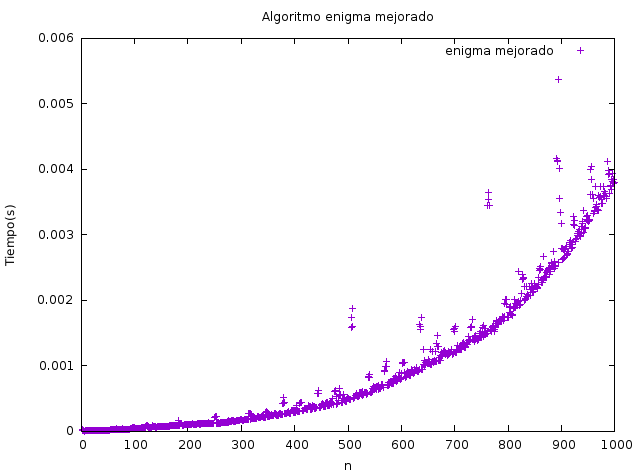
\includegraphics[scale=0.4, angle=0]{exp1.png}\end{center}
El siguiente gráfico muestra los resultados experimentales obtenidos del algoritmo enigma junto al algoritmo mejorado, ambos con el tamaño n de la matriz hasta 1000. 
\begin{center}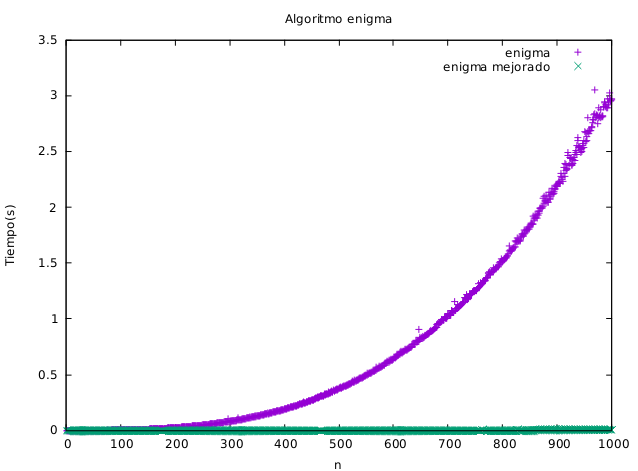
\includegraphics[scale=0.4, angle=0]{exp2.png}\end{center}


\section{Pregunta 2}
Suponga que se desea mantener un elemento en memoria con probabilidad uniforme sobre todos los elementos que vayan llegando de uno en uno. Esto se quiere hacer sin saber el número de elementos que llegará por adelantado. Se le pide escribir un algoritmo que realice esto,probando que la probabilidad de que un elemento cualquier que haya pasado pueda quedar en memoria sea efectivamente uniforme. Indicar su complejidad.\\
\subsection{Fundamento}
Sea $Memory[n]$ un arreglo de tamaño $n$ el cual está completo, y $A[m]$ un arreglo de elementos (procesos) que están en espera de ejecución. Se necesita liberar espacio dentro de $Memory$ de manera que cada elemento tenga igual probabilidad de salir, en efecto, realizaremos las combinaciones entre los $n-1$ elementos que están en memoria (el primer elemento por si solo tiene ventaja respecto del conjunto de procesos). Este proceso de selección comienza entre un par del arreglo y crece a medida que avanzamos en los elementos.\\
A continuación se muestra el funcionamiento del algoritmo. El arreglo inicialmente se encuentra completo. Sin embargo, para efectos de ver quien saldrá solo seleccionamos el primer elemento y luego iteramos.

\begin{center}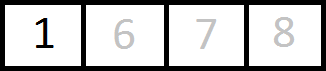
\includegraphics[scale=0.5, angle=0]{1.png}\end{center}
Para i = 1 y con la función Random oscilando en 1 valor, por lo tanto, \textbf{1 es seleccionado}.
\begin{center}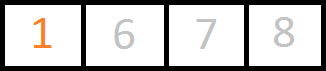
\includegraphics[scale=0.5, angle=0]{2.png}\end{center}
Luego para i=2 y con la funcion Random oscilando en 2 valores, tenemos
\begin{center}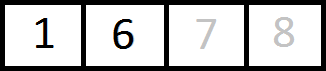
\includegraphics[scale=0.5, angle=0]{3.png}\end{center}
La funcion random saca un valor al azar entre \{1,2\}
\begin{center}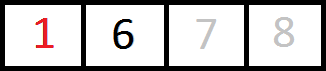
\includegraphics[scale=0.5, angle=0]{4.png}\end{center}
Vuelve a salir el 1, sin embargo, se mantienen la probabilidad individual de cada elemento cuando i = 2. A continuación, tomamos los 3 valores.
\begin{center}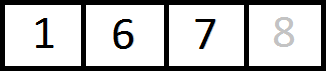
\includegraphics[scale=0.5, angle=0]{5.png}\end{center}
Se repite el procedimiento anterior, tomando como seleccionado un número aleatorio entre la cantidad de elementos comprendidos por i.
\begin{center}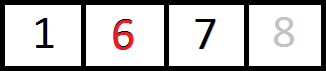
\includegraphics[scale=0.5, angle=0]{6.png}\end{center}
\begin{center}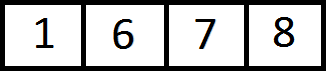
\includegraphics[scale=0.5, angle=0]{7.png}\end{center}
\begin{center}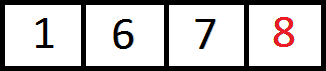
\includegraphics[scale=0.5, angle=0]{8.png}\end{center}
\subsection{Código}  
En la primera línea del pseudo-código seleccionamos el primer elemento (para el caso particular donde ingresa un solo proceso). Luego debemos considerar los elementos siguientes para verificar si son elegidos. De ocurrir esto último, $select$ pasa a tomar el valor de la posición i en esa iteración.\\
Continuando, volvemos a repetir el ciclo, esta vez con el siguiente elemento, y ademas se amplía el rango del $Random$.\\Finalmente retornamos la posición del proceso que debe salir de memoria.\\

\begin{algorithm}[H]

\caption{int select\_item(Array Memory[n], element)}
select $\leftarrow$ 0 \\

\For{$i=2$ to $n$}{r $\leftarrow$ Random( $1,..,i$ )\\
\If{r iqual i}{select $\leftarrow$ $i-1$} i++\\M[ select ] $\leftarrow$ element
}
\end{algorithm}

\subsection{Correctitud}
El algoritmo se encarga de insertar o expulsar elementos de un arreglo, garantizando además, que la probabilidad de que un elemento salga de la lista sea uniforme para todos los elementos.
\subsubsection{Demostración Correctitud}
Se define lo siguinte:

$\bullet$ \textbf{Pre-condición}: El algoritmo recibe una entrada de elementos, sin embargo, estos van entrando de uno.

$\bullet$ \textbf{Post-condición}: El algoritmo retorna la posición que se debe cambiar.\\

\textbf{Prueba:} Por cada iteración se asume que el arreglo está lleno por lo tanto debe salir un elemento.\\En cada ciclo entonces, se ejecutará la funcion random que entregará un numero al azar entre $1 ...i$. Mientras más elementos lleguen, más es el rango de posibilidades del Random.\\
Estos pasos continúan hasta que se termine de recorrer todo el arreglo de entrada y garantizar que todos han estado en igualdad de condiciones.\\Notemos que cada vez que ingresamos un nuevo elemento vemos la probabilidad de todos nuevamente, con ésto se mantiene la uniformidad.

\subsection{Demostración}
Para demostrar que \emph{la probabilidad de un elemento que haya quedado en memoria sea uniform}e, mostraremos que la probabilidad de salir es uniforme para cada elemento.\\ Consideremos $P\{X_i\}=\frac{1}{n}$ la probabilidad de salir de un elemento $X_i$. Luego por \textbf{inducción} tenemos que:
\begin{enumerate}
\item Para $n = 1$, la probabilidad de salir es $P\{X_i\}=\frac{1}{1} = 1$, por lo tanto, es claro que la probabilidad es uniforme para un elemento en particular.

\item Para $n$, sabemos que $P\{X_i\}=\frac{1}{n}$ es uniforme para cada $X_i$ en Memoria. $\models$ \textbf{Hipótesis de inducción}

\item Para $n+1$, utilizando la propiedad $P(A\bigcap B) = P(A)\ast P(B)$, entonces, la probabilidad de salir de un elemento $i$ que se encuentra dentro del arreglo completo es: $P\{X_i\}=\frac{1}{n}$.\\Por Hipótesis de inducción sabemos que $P\{X_i\}=\frac{1}{n}$ es uniforme $\bigvee i \in Memory$$[$ $]$. Para que ésto se mantenga debemos considerar la probabilidad de que el siguiente elemento $n+1$ no salga de memoria (pues ya sale uno anterior y debemos mantener la uniformidad). Luego tenemos que $P(X_n\bigcap \neg X_{n+1}) = P(X_n)\ast \neg P(X_{n+1})$ y la probabilidad de que el elemento $X_{n+1}$ no salga es $1-\frac{1}{n+1} \Rightarrow P'\{X_n\}=\frac{n}{n+1}$.\\ Finalmente,\\\\ $P(X_n\bigcap \neg X_{n+1}) \Leftrightarrow P(X_n)\ast \neg P(X_{n+1}) \Rightarrow \frac{1}{n} \ast (1-\frac{1}{n+1}) = \frac{1}{n+1}$\\\\Por lo tanto, se cumple para n+1 $\Rightarrow$ la probabilidad de salir de cada elemento es uniforme, y por complemento, \emph{la probabilidad de permanecer en memoria es uniforme}.
\end{enumerate}

\subsection{Complejidad Algorithm 2}
Para analizar la complejidad del algoritmo, definimos como \emph{operación básica} la llamada a \textbf{Random}, pues ésta se ejecutará un número considerable de veces que determinarán el comportamiento del algoritmo.
Nótese que las demás operaciones se asumen constante durante la ejecución. Así, el ciclo \textbf{for} determina que la función \textbf{Random} se ejecutará $n-1$ veces puesto que el primer elemento queda seleccionado desde un comienzo.\\

\begin{center}$\sum_{i=2}^{n}1 = 1 + 1 + ... + 1 = n + c$\end{center}
Luego, para m operaciónes de inserción debemos ejecutar el algoritmo. Por lo tanto:\\
\begin{center}$T(m) = m \ast n$\end{center} Donde $T(m)$ es el tiempo que demorá el algoritmo en ejecutar $m$ inserciones en un arreglo de tamaño $n$. Vemos que el tamaño del arreglo es independiente de las m inserciones y se mantendrá constante durante la ejecución. Por lo tanto, \\\begin{center}$T(m) = km$\end{center}.
Si analizamos el comportamiento asintótico de la función podemos decir,\\
\begin{center}¿ \(km \in \Theta(m) \) ?\end{center}
Por definición,\begin{center}$0 < c_1m \leq km \leq c_2m$ \end{center}
Luego, para $\forall m,$ $m\geq 0$, es claro que, $c_1\leq k \leq c_2$.

\section{Conclusión}
El seguimiento del primer algoritmo nos permitió definir un algoritmo mas eficiente, cuyos resultados experimentales favorecieron mucho al proceso en general. Se pudo comprobar teórica y prácticamente el algoritmo propuesto. \\Por otro lado, el segundo problema nos permitió crear un algoritmo que efectivamente mantenía la probabilidad del suceso en estado uniforme.\\Para ambos problemas, las cotas no estaban delimitadas por el mejor y peor caso, ya que estás no variaban en resultado y eran las entradas las que condicionan el curso del programa. 



\end{document}
